\documentclass[10pt]{article}
\usepackage[sc]{mathpazo}
\usepackage{commands}
\hypersetup{colorlinks = true}
\let\oldphi\phi 
\let\phi\varphi 
\let\varphi\oldphi



\begin{document}
\begin{tcolorbox}
  \begin{center}
  \begin{Large}
    \textbf{Introduction to Solid State Physics Notes} \\
    \vspace{5pt}
  \end{Large}
  \begin{large}
        Tobias Faehndrich \\
\vspace{5pt}
    \emph{This document was typeset on \today}
  \end{large}
  \end{center}
\end{tcolorbox}

\begin{center}
  \textbf{Introduction:}

Notes written while following the upper-level undergraduate course taught at the University of Pittsburgh in the Fall 2015 semester by Sergey Frolov. The course is based on Steven Simon's "Oxford Solid State Basics" textbook. If any errors are found in the notes, feel free to email me at \href{mailto:tobias.faehndrich@gmail.com}{tobias.faehndrich@gmail.com}. Overleaf formatting was copied from Rio W.

\end{center}
\addtocontents{toc}{\protect\hypertarget{toc}{}}
\tableofcontents


\newpage

\setcounter{section}{1}

\section[Quantum Review]{\hyperlink{toc}{Quantum Review}}

\begin{itemize}
    \item Harmonic oscillator distance between energy levels is always the same.
    \item wavefunctions allows for tail going past classically allowed area.
    \begin{itemize}
        \item exponential decay
    \end{itemize}
    \item \textbf{Particle in a Box (PIB)}
    \[E = \frac{n^2\hbar^2}{8mL^2}, \qquad n = 1,2,3...\]
    \[\Delta E = (2n+1) \frac{\hbar^2}{8mL^2}\]
    \item \textbf{Harmonic Oscillator (HO)}
    \[E = \hbar \omega (\frac{1}{2} + n), \qquad n=0,1,2,3...\]
    \[\Delta E = \hbar \omega\]
    
    \item \textbf{Coulomb Potential (Hydrogen 1p+1e)}
    \[ U(r) = \frac{-e^2}{4\pi \epsilon_0 r}\]
    \begin{itemize}
        \item \[\Psi(r)\Phi(\theta,\phi)\]
    \end{itemize}
    \item eigenvalues are possible energies
    \item radial quantum number $n_r = 0,1,2...$
    \item principle quantum number $n \equiv n_r + l + 1$
    \item S family orbitals (l=0)
    \item 2 types of particles that make large differences in behaviour @ $T=0$ and low $E$.
    \begin{enumerate}
        \item \textbf{Bosons:}
        \begin{itemize}
            \item occupation number can take any value 
            \item ex: photons, mesons, composite particle with integer spin (ex. Li$^7$)
            \item even total number of proton/electron/neutron
        \end{itemize}
        \item \textbf{Fermions:}
        \begin{itemize}
            \item occupation number can be zero or one (Pauli exclusion principle).
            \item ex. electrons, protons, neutrons, composite particles with half-integer spin
            \item odd number of proton/electron/neutron
        \end{itemize}
    \end{enumerate}
    \item  
    \[\beta = \frac{1}{kT}\]
    \[\bar{n}_s = \frac{1}{exp(\beta(\epsilon_s-\mu))-1}\]
    \begin{figure}
        \centering
        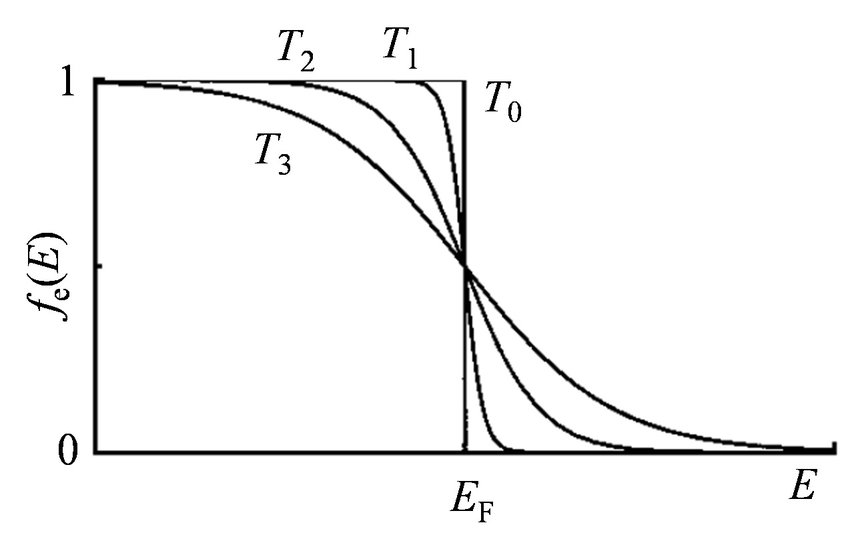
\includegraphics[width=0.5\linewidth]{Images/Fermi-Dirac-distribution.png}
        \caption{Temperature dependence of Fermi-Dirac distribution}
        \label{fig:Fermi-Dirac}
    \end{figure}
\end{itemize}


\newpage
\section[Einstein $\&$ Debye Models of a solid]{\hyperlink{toc}{Einstein $\&$ Debye Models of a solid}}


\begin{itemize}
    \item \textbf{Heat Capacities of Solids:}
    \begin{itemize}
        \item rate of change of energy with temp (@const Volume)
        \[C = \frac{dE}{dt} \]
        \item @ $T \gg 0 , \qquad C=3Nk$
        \item Law of Dulong $\&$ Petit
        \item Classically: Law of equipartition
        \begin{itemize}
            \item $C=\frac{k}{2}$ for each DOF in material.
        \end{itemize}
        \item $C_V \propto \alpha T^3 + \gamma T$
        \begin{itemize}
            \item Insulators: $\gamma=0$
            \item Conductors: $\gamma\neq0$
        \end{itemize}
    \end{itemize}
    \item \textbf{Einstein model of Solid}
    \begin{itemize}
        \item each atom in crystal vibrates independantly
        \item assumed these were Harmonic Oscillators $E_n=\hbar \omega_E(n+\frac{1}{2})$
        \item partition function
        \[Z = \frac{exp(-\beta \hbar \omega_E /2}{1-exp(-\beta\hbar\omega_E)}\]
        \[Z = \sum_r exp(-\beta E_r) \]
        \[\bar{E} = -\frac{1}{Z} \frac{dZ}{dB} \]
        \[ C_V = \left(\frac{\partial \bar{E}}{\partial T}\right)_V \]
        \item Result
        \[C_V=3Nk(\beta \omega_E \hbar)^2 \frac{e^{\beta \hbar \omega_E}}{(e^{\beta \hbar \omega_E}-1)^2}\]
        \item $T\rightarrow \infty , \qquad C_V = 3Nk$ 
        \item $T\rightarrow 0, \qquad C_V = 0 $
        \item real solids go $T^3$ instead of exponentially
        \item partially successful model $\rightarrow$ shape behaviour @ low temp was incorrect.
    \end{itemize}
    \item \textbf{Debye's Model}
    \begin{itemize}
        \item atoms coupled to each other in a solid
        \item atoms vibrations generate sound waves
        \item quantize! (can use planck's results for light quantization)
        \item "phonons" vs photons
        \begin{itemize}
            \item described by wavevector k
            \item longitudinal and transverse modes possible for phonons
        \end{itemize}
        \item Debye Temp $\theta = \frac{\hbar \omega_D}{k}$
        \[C_V = \frac{12\pi^4}{5}Nk\left(\frac{T}{\theta_D}\right)^3\]
        \[E~T^4 \qquad \therefore C_V~T^3\]
        \item still not fully complete
    \end{itemize}
\end{itemize}



\newpage
\section[Drude $\&$ Sommerfeld Theories of electrons in solids]{\hyperlink{toc}{Drude $\&$ Sommerfeld Theories of electrons in solids}}


\begin{itemize}
    \item \textbf{Drude (1900):} kinetic gas, classical ideas
    \begin{itemize}
        \item \textbf{Principles of Drude Theory:}
        \begin{enumerate}
            \item electrons have an avergae scattering time $\tau$.
                $\rightarrow$ phenomenological parameter (based on observable facts)
            \item after scattering event occurs, electron returns from some p to momentum p=0.
            \item \[F=-e(\vec{E} + \vec{v}\times\vec{B})\]
            Between events, electron responds as a free particles to applied $\vec{E} \& \vec{B}$ fields.
        \end{enumerate}
        \item \textbf{Steady State:} $\frac{dp}{dt}=0$
        \begin{itemize}
            \item \textbf{conductivity:} \[ \sigma = \frac{ne^2\tau}{m} \]
            from current density
            \[\vec{j} = \sigma E \]
            \item \textbf{resistivity:}
            \begin{itemize}
                \item \[\rho = \frac{m}{ne^2\tau} \] 
            \end{itemize}
        \end{itemize}
        \item \textbf{With Magnetic Field:} In semiconductor m $\rightarrow$ m* (mass is replaced by an effective mass).
        
        "non-local" \[V_y = \rho_{xy} I_x \] 
        "local" \[V_x = \rho_{xx} I_x \] 
        Hall coefficient\[R_H = \frac{\rho_{xy}}{|B|} = - \frac{1}{ne} \]
        
    \end{itemize}
    \item \textbf{Sommerfeld theory (1920):} assumed fermionic behaviour
\end{itemize}



\newpage
\section[1D models of vibrations]{\hyperlink{toc}{1D models of vibrations}}

\begin{itemize}
    \item monatomic chain (restricted to longitudinal motion for now.)
    \item a: lattice constant and k: spring constant
    \item equilibrium position for the nth atom and displacement.
    \[x_n^{eq}= na\]
    \[\delta x_n = x_n - x_n^{eq}\]
    \item Hooke's Law:
    \[F_n = k( \delta x_{n+1} - \delta x_n)-k(\delta x_n - \delta x_{n-1})\]
    \item Newton's Law $\rightarrow$ equations of motion (EoM) make ansatz:
    \[\delta x_n = A e^{-ikna + i \omega t} \] 
    \item Plug ansatz into Newton:
    \[ \omega = 2 \sqrt{\frac{k}{m}\left| \sin\left(\frac{ka}{2}\right)\right|} \]
    \item A: amplitude and k: wave vector (related to momentum).
    \item Point with k=0; Reciprical Lattice points $G_m$ and Positions of atoms of along the chain $x_n$.
    \[G_n = \frac{2 \pi n}{a} , \qquad n = -2,-1,0,1,2,...\]
    \item Reciprocal lattice $\leftrightarrow$ Direct lattice
    \item
    \[e^{iG_m x_n} = 1 \]
    \item 1st Brillouin Zone: unit cell centered around k=0 with boundaries @ $k= \pm \frac{\pi}{a}$ in reciprocal lattice. All allowed cases contained in 1st. 2nd 3rd etc can be helpful but not needed.
    \item for finite length: 
    \[k=\frac{2\pi n}{L} \] 
    \textbf{Phonons}
    \[E_n = (\frac{1}{2}+n)h\omega \]
    \item each excitation of harmonic oscillators corresponding to vibrations in a material $\rightarrow$ bosons (which phonons are).
    
    \item number of phonons is $\therefore$ given by Bose distribution.
    \[n_B (\beta \hbar\omega) = \frac{1}{e^{\beta \hbar\omega} -1 } \]
    \item Diatomic chain + excitations with multiple branches
    $\rightarrow$ leads to increase in possible modes of vibrations.
    \item Again assume coupled according to Hooke's Law (and easier if we let m1=m1)
    \item Sol. Newton:
    \[\begin{cases}
      m \frac{d^2(\delta x_n)}{\partial t^2} = k_2 (\delta y_n - \delta x_n)+ k_1 (\delta y_{n-1} - \delta x_n)\\
      m \frac{d^2(\delta y_n)}{\partial t^2} = k_2 (\delta x_n - \delta y_n)+ k_1 (\delta x_{n} - \delta y_n)
    \end{cases} \]
    \item Ansatz:Plug into the matrix form of EoM.
    \[\begin{cases}
    \delta x_n = A_x e^{-ikna+i\omega t} \\
    \delta y_n = A_y e^{-ikna+i\omega t}
    \end{cases}\]
    \item solve for $\omega$. plus or minus solutions or multiple solutions will give a E-k diagram and thus the Single Brillouin Zone. The top one in this case is Optical phonons and the bottom is Acoustic phonons (which are nuanced names. Photons can interact only with the "optical" phonons. 
    \[\omega = 2 \sqrt{\frac{k}{m}} \left| \sin\left(\frac{ka}{2}\right)\right| \]
    \begin{figure}
        \centering
        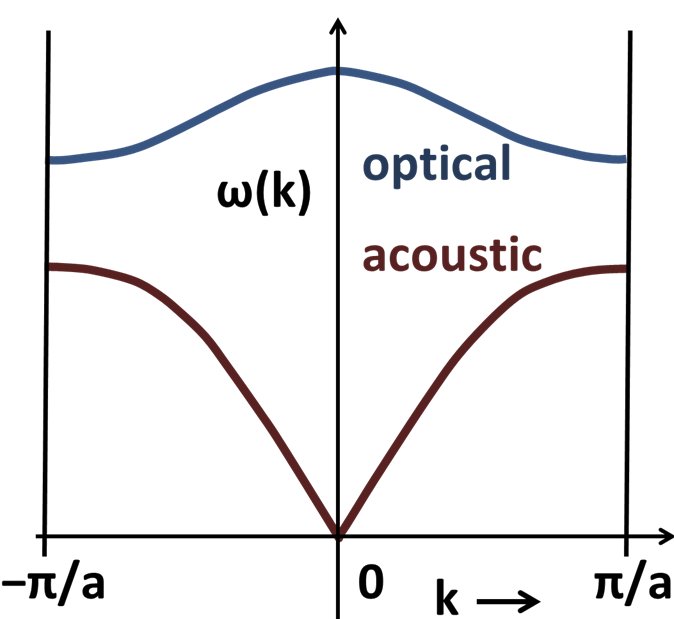
\includegraphics[width = 0.5\linewidth]{Images/phonon_modes.png}
        \caption{Caption}
        \label{fig:phonon modes}
    \end{figure}
    \item \textbf{Extended zone scheme}
    \begin{itemize}
        \item shifts the optical to the second brillouin zone and leaves the acoustic in the first.
        \item makes it easier to see the change from diatomic to monatomic.
        \begin{figure}
            \centering
            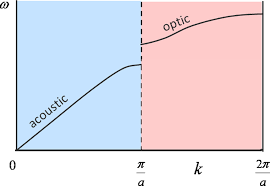
\includegraphics[width = 0.5\linewidth]{Images/extended_zone_scheme.png}
            \caption{extended zone scheme}
            \label{fig:extended zone scheme}
        \end{figure}
    \end{itemize}
\end{itemize}




\newpage
\section[The 1D Tight Binding Model for Electrons]{\hyperlink{toc}{The 1D Tight Binding Model for Electrons}}


 \begin{itemize}
     \item "Hopping of an electron along a 1D lattice.
     \item each atom has 1 orbital denoted by $\ket{n}$
     \begin{itemize}
         \item orthogonal to eachother $\Braket{n|m} = \delta_{n,m}$ although the true Kronecker-Delta function result is only really true if the atoms are far enough away from each other.
     \end{itemize}
     \item Wave function of the electron in the basis of the orbitals is:
     \[\ket{\Psi} = \sum_n c_n \ket{n} \]
     \item Model of linear combination of atomic orbitals (LCAO) 
     \item Time Independent Schrodinger Equation (TISE):
     \[ H \ket{\Psi} = E \ket{Psi}\]
     \item Hamiltonian only couples nearest neighbour sites so we say:
     \[ \braket{n | H | m} = \begin{cases}
     \epsilon_0, \qquad n=m \leftarrow \text{staying in atom} \\
     -J, \qquad n=m\pm1  \leftarrow \text{ hop by 1 site is way more probable} \\
     0, \qquad \text{otherwise} \leftarrow \text{than hopping by severeal atoms.}
     \end{cases}\]
     
     \[ \braket{n | H | m} = \begin{bmatrix} 
    \epsilon & -J & &\text{\huge0} &\\
    -J & \epsilon & -J & & \\
    & -J & \ddots & \ddots & \\
    \text{\huge0} & & \ddots & &
    \end{bmatrix}
    \]
    \[ \braket{n|\mathcal{H}|m} = \epsilon_0 \delta_{n,m} - J(\delta_{n,m+1} + \delta_{n, m-1})\]
    \[ \sum_m H_{n,m} c_m = E c_n \]
    TISE: \[ \epsilon_0 c_n - J (c_{n-1} + c_{n+1}) = E c_n\]
    Plug-in Ansatz (without time dependancy): \[ c_n = \frac{e^{-ikna}}{\sqrt{N}} \] 
    Relationship to phonons -- obtain disperesion relation:
    \[ E = \epsilon_0 - 2J \cos(ka) \]
    We get single band because we chose to have 1 orbital per site with our current model.
    \item \textbf{Phonons} in \textbf{monatomic chain} $\rightarrow$  \textbf{ diatomic or more complex crystals} \\
    \vspace{7px}
    similar to 
    \item \textbf{Band Diagram} in \textbf{1 orbital per site} $\rightarrow$ \textbf{multiple orbitals per site}
    \item We can represent \textbf{band structure} (energy ranges and k-dependence of multiple bands.
    \item Reduced zone scheme vs Extended zone scheme
    \begin{figure}
        \centering
        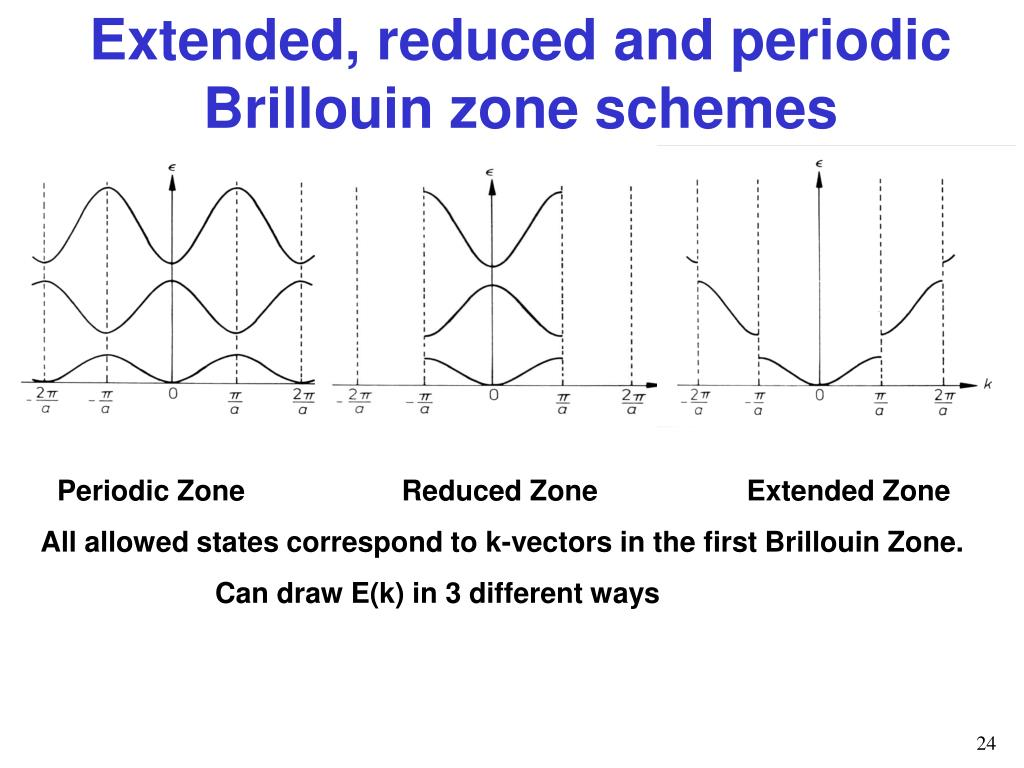
\includegraphics[width = 0.75 \linewidth]{Images/extended-reduced-and-periodic-brillouin-zone-schemes-l.jpg}
        \caption{Caption}
        \label{fig:brillouin zone}
    \end{figure}
    \item Typically many bands in solids with 2 relevant bands
    \item no solutions for any energy in this gap which relates to insulators, conductors, semiconductors etc.
    \item energy gap = band gap, and occurs at edge of Brillouin zone for the extended zone scheme.
    \item \textbf{Bandwidth} effective mass and crystal momentum
    \item width of the band energy depends of nuclei spacing
    \item N lattice sites + one orbital $\rightarrow$ N states for electron.
    \item $\frac{2 \pi}{aN}$ spacing is so incredibly small for all particle solids so we therefore assume band structure is continuous.
    \item \textbf{Band Shape}\\
    Approximate for $k\ll 1$ we see parabolic near k=0 for free particle $E=\frac{p^2}{2m} = \frac{\hbar^2k^2}{2m}$.
    \[E = \epsilon_0 -2J \cos(ka)\]
    \[E \approx \epsilon_0 - 2J(1-\frac{(ka)^2}{2})\]
    \[E \approx \epsilon_0 -2J + Ja^2k^2 \]
    \[E = \frac{\hbar^2 k^2}{2m^*}+ \text{Const.}\]
    \[\frac{\hbar^2 k^2}{2m^*} = Ja^2 k^2 \]
    Effective Mass (determined by J: hopping parameter/ tunnelling amplitude):
    \[ m^* = \frac{\hbar^2}{2Ja^2} \]
    \textbf{Filling Bands and the Fermi Surface}
    \item atoms with one valence electron, expect donate to collection moving in band.
    \item electrons have 2 spin ($\uparrow$, $\downarrow$) which gives room for 2N electrons in band.
    \item at low temp ($ T \ll T_f$), half filled band involves states being filled up to the Fermi Energy.
    \item system has fermi surfaces (here only 2 points) k points where the filled meets unfilled region.
    \item c $\propto$ T: heat capacity propto temp
    \item \textbf{Metal}: the fermi surface is in the middle of a band.
    \item applied external electrical field, electrons can accelerate to higher values of k $\rightarrow$ current flows in material. (backward and forward moving).
    \item \textbf{Band Insulator}: if band is filled, fermi surface is at the edge of the Brillouin Zone, then there are no states available in band for electrons to move into by an electrical field. (almost never carries current)
    \item \textbf{Energy Gap} \\
    $\rightarrow$ if it's large enough it's snot possible for electron to be pushed to higher band.\\
    $\rightarrow$ if BG $\ge 4eV$ then material is an (band) insulator.\\
    $\rightarrow$ if BG $<$ 4eV then electrons can be transferred to higher bands either @ \textbf{finite temperatures} or with \textbf{applications of fields} $\rightarrow$ material can then be a semiconductor.
    \item Many materials with \textbf{2 valence electrons} are insulators $\rightarrow$ some can form metals if interatomic spacing is small enough (two bands merge). See E bands vs atomic spacing.
    \item \textbf{Opposite} many materials with 1 valence electron are metals $\rightarrow$ some are special type of Insulator: "Mott Insulator"
    \item too much energy to have 2 electrons (ex. NiO $\&$ CoO) on one site.
    \item Simple band model also doesn't fully describe when system has magnetic properties (ferro, antiferro, $\&$ ferro) spin alignment.
    \item kwant simulation library in PYTHON is a cool resource.
 \end{itemize}



\newpage
\section[Crystal Structure]{\hyperlink{toc}{Crystal Structure}}


\begin{itemize}
    \item crystals: periodic arrangements of atoms in a lattice
    \item Penrose tyles are quasi crystal.
    \item \textbf{Lattice:} repeating structure defined as an infinite set of points, which can be constructed as sums of set of linearly independent \textbf{primitive lattice vectors}.
    \[ \vec{R} = n_1 \vec{a}_1 + n_2 \vec{a}_2 + n_3 \vec{a}_3, \qquad n \in \{0, \pm1, \pm2 ...\} \]
    \item Points in the form of: $2\vec{a}_1 + \vec{a}_2$ notated as $[2,1]$
    \item \underline{Square Lattice:} $\phi = 90^{\degree}, \qquad |a_1|=|a_2|$
    \item \underline{Hexagonal Lattice} (or Triangular): $\phi = 120^{\degree}, \qquad |a_1|=|a_2|$
    \item choice of primitive lattice vectors for a lattice is not unique $\rightarrow$ must be able to get to any spot/point on the lattice with a linear combination.
    \item \textbf{Unit cell:} a region of space chosen so that you could tile/ fill all of space.
    \item \textbf{Primitive Unit Cell:} Unit cell with exactly one lattice point inside (conventional/convenient unit cell is when it is not primitive). Can also add fractions of points to add up to 1 full point for PUC (i.e. $4 * 1/4 = 1$).
    \item \textbf{Wigner-Seitz Unit Cell:} is a way to construct a primitive unit cell that is always possible.
    \begin{enumerate}
        \item Draw lines to connect a given lattice point to all nearby lattice points
        \item At the midway points, normal to these lines, draw new-lines or planes.
        \begin{itemize}
            \item (smallest volume enclosed in this way is the Wigner-Seitz primitive cell. All space may be filled by these cells.)
            \item \textbf{notice}: not all lines from the method need to be used in the end.
        \end{itemize}
    \end{enumerate}
    \item \textbf{Crystal with Multiple Atom Types:}
    \begin{itemize}
        \item Unit cell can have more than one atom
        \item periodic for each atom type or for some region in space repeated periodically.
        \item Define a basis for example for the large atom and for the small atom.
    \end{itemize}
    \item \textbf{Simple Cubic 3D:} very improbable in nature cause there is so much empty space where crystal could configure in a more efficient manner.
    \begin{itemize}
        \item can be \textbf{unit cell (a), tetragonal $(a = b \neq c)$ or orthorhombic $(a \neq b \neq c)$}
    \end{itemize}
    \item Cesium Chloride (CsCl): is simple cubic with basis Cs [0,0,0] and Cl [1/2, 1/2, 1/2]
    \item \textbf{Unit Cell of Body Centered Cubic Lattice (BCC):}
    \begin{itemize}
        \item Much more probable 
        \item Simple cubic with basis also Body centered cubic (BCC):
    \end{itemize}
    \item \textbf{Face Centered Cubic (FCC):}
    \begin{itemize}
        \item nature likes even more (probable!), for ex: NaCl Salt or C Diamond.
    \end{itemize}
    \item The full list of all possible 3D crystal types (\textbf{The 14 Bravais Lattice Types})
    \begin{itemize}
        \item \textbf{4 types of Unit Cells }
        \begin{itemize}
        \item P = primitive
        \item I = Body-centered
        \item F = Face-centered 
        \item C = side-centered
        \end{itemize}
        \item \textbf{with 7 crystal classes}
        \begin{enumerate}
            \item Cubic
            \item Tetragonal
            \item Orthorhombic
            \item Hexagonal
            \item Trigonal
            \item Monoclinic 
            \item Triclinic
        \end{enumerate}
    \end{itemize}
    \item GaAs is a zincblende FCC Basis atom1 (0,0,0) and atom2 (1/4, 1/4, 1/4).
\end{itemize}

\newpage
\section[Reciprocal Lattices]{\hyperlink{toc}{Reciprocal Lattices}}

space in which waves live

not only electron or vibrational waves
-- also waves of light travelling through a crystal

X-rays are used very often to study crystals

\textbf{Recall Reciprocal Lattice in 1D}

\[\sigma x_n = Ae^{i\omega t - i k n a} \]

where:

a = lattice const (direct, in real space)

any system that is periodic in space (a) is also periodic in k space (or reciprocal space) with period $2\pi/a$

Points equivalent to k=0:

\[G_n = \frac{2\pi n}{a}\]

 where n = ... -2, -1, 0, 1, 2, ...
 
 \begin{center}
\begin{tabular}{|c c c c c c c c|} 
 \hline
 \textbf{Space} & ... & n=-2 & n=-1 & n=0 & n=1 & n=2 & ...  \\ [0.5ex] 
 \hline\hline
 $x_n$ =  & ... & -2a & -a & 0 & a & 2a & ... \\ 
 \hline
 $G_n$ =    & ... & -2($\frac{2\pi}{a}$) & -($\frac{2\pi}{a}$) & 0 & ($\frac{2\pi}{a}$)  & 2($\frac{2\pi}{a}$) & ... \\ [1ex] 
 \hline
\end{tabular}
\end{center}


We find a relationship between the spaces:

\begin{tcolorbox}[enhanced,attach boxed title to top center={yshift=-3mm,yshifttext=-1mm},
  colback=blue!5!white,colframe=blue!75!black,colbacktitle=red!80!black,
  title=Reciprocal-Direct Lattice Relationship,fonttitle=\bfseries,
  boxed title style={size=small,colframe=red!50!black} ]
  \begin{equation}
      e^{iG_mx_n} = 1
  \end{equation}
\end{tcolorbox}

\textbf{Reciprocal Lattice now in 3D}

Real:

\[ \textbf{R} = n_1\textbf{a}_1 + n_2\textbf{a}_2 + n_3\textbf{a}_3, \qquad n_i \in  \{0,\pm1, \pm2, \pm3, ...\} \]
 
 Reciprocal:

\[ \textbf{G} = m_1\textbf{b}_1 + m_2\textbf{b}_2 + m_3\textbf{b}_3, \qquad m_i \in  \{0,\pm1, \pm2, \pm3, ...\} \]


Conditions to find vectors of the reciprocal lattice:
\begin{equation}
    e^{\textbf{G}\cdot \textbf{R}} = 1
\end{equation}

construct primitive lattice vectors for the reciprocal lattice \textbf{$b_i$}, using the property that
\begin{equation}
    \textbf{a}_i \cdot \textbf{b}_j = 2 \pi \delta_{ij}
\end{equation}


Ways to determine the reciprocal lattive vectors:
\begin{itemize}
    \item Using a Fourier Transformation of the original lattice (not so intuitive):

\[\rho(x) = \sum_{n} \delta(x-na)\]
\[\mathcal{F}(\rho(x))= \int dx e^{ikx} \rho(x)\]
\[= \sum_n e^{ikan} \]
\[=\frac{2\pi}{a} \sum_m \delta \left(k-\frac{2\pi}{a}m\right) \]


\item Geometric Interpretation: see it as the set of vectors that are normal to the families of lattice planes (infinite set of equidistant parallel lattice planes which as a family contain all of the points of the lattice).

7\item Mathematical Way (minute 1:10 on L8 YT)

Must be equidistant planes and must include ALL points in a crystal.

\pagebreak


\begin{figure}
  \centering
  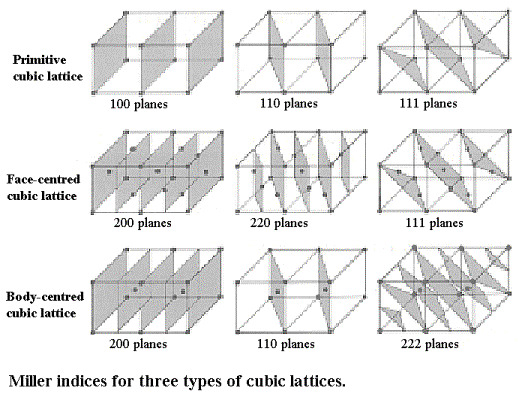
\includegraphics[width=0.6\linewidth]{Images/latticeplanes.jpg}
  \caption{Lattice Planes}
  \label{fig:Lattice Planes}
\end{figure}



\end{itemize}

\textbf{Family of latticce planes:} an infinite set of equidistant parallel lattice planes, which as a family contain all of the points of the lattice.

No extra planes can occur.

\textbf{Index System for Crystal Planes -- Miller Indices}:

\begin{enumerate}
    \item Express the intercepts of the plane with the crystal axes in units of lattice constants a1, a2, a3.
    \item Take the reciprocal of these numbers.
    \item Reduce them to integers of the same ratio: (h,k,l).
\end{enumerate}

\begin{itemize}
    \item round brackets () - reciprocal space
    \item square brackets [] - real space
\end{itemize}

\begin{itemize}
    \item plane parallel to an axis will result in a 0 in the Miller Indices
\end{itemize}

For some experiments it is important to know the distance between the lattice planes

General Distance formula:
\begin{equation}
    d_{hkl} = \frac{n}{\sqrt{\frac{h^2}{a^2}+\frac{k^2}{b^2}+\frac{l^2}{c^2}}}
\end{equation}
Distance for cubic lattice (simpler):
\begin{equation}
    d = \frac{a}{\sqrt{h^2+k^2+l^2}}
\end{equation}

\begin{itemize}
    \item bar over top of miller indice indicates negative number; ex ($11\bar{2}$)
\end{itemize}

\begin{figure}
  \centering
  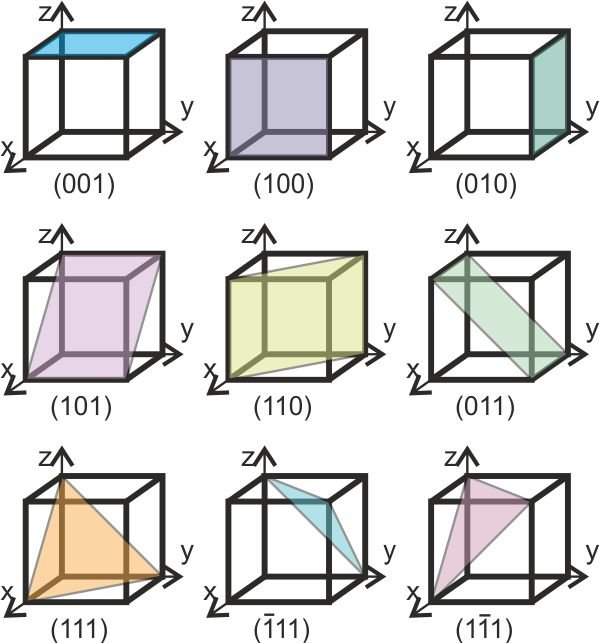
\includegraphics[width=0.6\linewidth]{Images/miller-indices.png}
  \caption{miller indices}
  \label{fig:Miller-Indices}
\end{figure}


\newpage
\section[Scattering Experiments (X-ray diffraction)]{\hyperlink{toc}{Scattering Experiments (X-ray diffraction)}}

~ Shining of wave on a crystal and detecting the scattered particles/radiation

- x-rays, electrons and neutrons

- wavelength of radiation should be comparable to a typical inter atomic distance of a few $\text{\AA}$.

\[E = h\nu = \frac{hc}{\lambda}\]

\[ \lambda(\text{\AA}) = 12398/E(eV)\]

- a few keV is needed for a wavelength of around 1 angstrom.

\textbf{X-Ray}
\begin{itemize}
    \item $\lambda = 1 \text{\AA}$
    \item E ~ $10^4 eV$
    \item interact with electron
    \item penetrating
\end{itemize}
\textbf{Neutron}
\begin{itemize}
    \item $\lambda = 1 \text{\AA}$
    \item E ~ $0.08 eV$
    \item interact with nuclei
    \item Highly penetrating
\end{itemize}
\textbf{Electron}
\begin{itemize}
    \item $\lambda = 2 \text{\AA}$
    \item E ~ $150 eV$
    \item interact with electron
    \item Less penetrating
\end{itemize}

- X-ray is great for bulk investigation
- Electron is great for surface investigation (checking surfaces with MBE)



\begin{tcolorbox}[enhanced,attach boxed title to top center={yshift=-3mm,yshifttext=-1mm},
  colback=blue!5!white,colframe=blue!75!black,colbacktitle=red!80!black,
  title=The Bragg Law,fonttitle=\bfseries,
  boxed title style={size=small,colframe=red!50!black} ]
  \begin{equation}
      2d\cdot\sin(\theta) = m\lambda 
  \end{equation}
\end{tcolorbox}

- Ignores some things but gives a good rough estimate with a simple model

- Diffraction occurs for:

\[ \vec{k} + \vec{G} = \vec{k}' \]

The larger the indices, the smaller the spacing between the planes.

- Single slit diffraction gives Fraunhover Diffraction Pattern
- This is a Fourier transform of the slit (or periodic crystal structure)

-   Atomic Form Factor increases with atomic charge.

- Some planes are absent in X-ray diffraction and some show:

The missing orders follow rules depending on which type of lattive it is -- 
\begin{itemize}
    \item \textbf{Simple Cubic (sc):} any (hkl)
    \item \textbf{Body-centred cubic (bcc):} h+k+l=even
    \item \textbf{Face-centred cubic (fcc):} h, k and l all odd or all even.
    
\end{itemize}
\begin{tabular}{ |p{3cm}||p{3cm}|p{3cm}|p{3cm}|  }
 \hline
 \multicolumn{4}{|c|}{\textbf{Lattice Type}} \\
 \hline
 Miller Indices & sc (P) & bcc (I) & fcc (F)\\
 \hline
 100 & Y & N & N\\
 110 & Y & Y & N\\
 111 & Y & N & Y\\
 200 & Y & Y & Y\\
 210 & Y & N & N\\
 211 & Y & Y & N\\
 220 & Y & Y & Y\\
 310 & Y & Y & N \\
 311 & Y & N & Y \\
 \hline
\end{tabular}

N = will not give a diffraction pattern for these planes (due to interference).
Y = will give ...

\textbf{X-Ray Diffraction (XRD) Methods:}
\begin{itemize}
    \item Laue: not that good
    \item Rotatin Crystal: meh
    \item Powder: to get lattice parameters, polycrystal (powdered), monochromatic beam, variable angle.
    \begin{itemize}
        \item Debye-Schenner cone
        \item beam comes through holes
    \end{itemize}
\end{itemize}


\textbf{XRD Procedure}
\begin{itemize}
    \item Measure angle 
    \item $d = \frac{\lambda}{2\sin\theta}$
    \item bigger angle gives smaller d
    \item small d corresponds to higher miller indices
    \item scale d's by the first one (get d=1 for first)
    \item scale all d by an clever choice of integer N
    \item $N = h^2 + k^2 + l^2 $
    \item {hkl}
    \item $a = d \sqrt{h^2 + k^2 + l^2}$ (hopefully getting the same a for all)
    \end{itemize}

\begin{tabular}{ |p{2cm}|p{3cm}|p{2cm}|p{1.5cm}|p{1.5cm}|p{1.5cm}|  }
 \hline
 \multicolumn{6}{|c|}{\textbf{Scattering Selection Rules}} \\
 \hline
{hkl} & $N=h^2+k^2+l^2$ & Multiplicity & sc (P) & bcc (I) & fcc (F)\\
 \hline
 100 & 1 & 6        & * &   &  \\
 110 & 2 & 12       & * & * &  \\
 111 & 3 & 8        & * &   & *\\
 200 & 4 & 6        & * & * & *\\
 210 & 5 & 24       & * &   &  \\
 211 & 6 & 24       & * & * &  \\
 --- & 7 & --       &   &   &  \\
 220 & 8 & 12       & * & * & *\\
 221,300 & 9 & 24+6 & * &   &  \\
 310 & 10 & 24      & * & * &  \\
 311 & 11 & 24      & * &   & *\\
 222 & 12 & 8       & * & * & *\\
 320 & 13 & 24      & * &   &  \\
 321 & 14 & 48      & * & * &  \\
 --- & 15 & --      &   &   &  \\
 400 & 16 & 6       & * & * & *\\
 \hline
\end{tabular}

\textbf{XRD Identification of SC,BCC, FCC:}
\begin{itemize}
    \item P (SC): N = 1,2,3,4,5,6,8,9,... (=all integers excluding 7,15,23,...)
    \item I (BCC): N = 2,4,6,8,10,12,14,... (=even integers excluding 28, 60,...)
    \item F (FCC): N = 3,4,8,11,12,16,19,20,...
\end{itemize}


\begin{figure}
  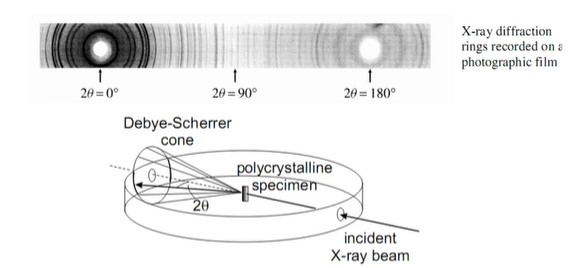
\includegraphics[width=0.75\linewidth]{Images/XRD.jpg}
  \caption{XRD}
  \label{fig:XRD}
\end{figure}


\newpage
\section[Electron waves in crystals]{\hyperlink{toc}{Electron waves in crystals}}

Multiplicity: some families of lattice planes have the same spacing, and thus would in indistinguishable in an XRD experiment.

\begin{figure}
  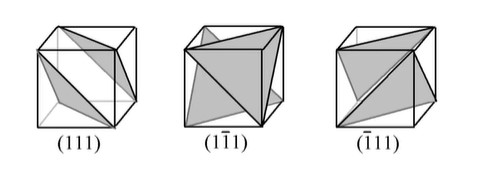
\includegraphics[width=0.75\linewidth]{Images/111 class.jpg}
  \caption{111}
  \label{fig:111}
\end{figure}

ex: {111} signifies all (111) (1$\bar{1}$1) and ($\bar{1}$11) in the so called '111' class. They all diffract with the same angle and thus the line will have a stronger intensity reading compared to other classes without the negative miller indices.

Most common basis structure is sodium chloride NaCl and zinc blende ZnS.

- you can use pattern in XRD or neutron scattering data (i.e. odd peaks (h+k+l=odd) are big and even are small) can tell you which basis it is from.

\textbf{Refresher of Brillouin Zones}

\begin{figure}
  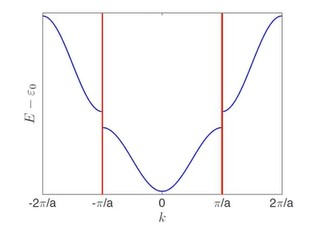
\includegraphics[width=0.75\linewidth]{Images/BrillouinZone.jpg}
  \caption{BZ}
  \label{fig:BZ}
\end{figure}

- You can perform Wigner-Seitz (closest lines drawn, then half way points draw perpendicular lines/planes) method to find 1st,2nd,3rd, etc Brillouin Zones on a lattice.
- first is for the reciprocal lattice point G=0.

\begin{figure}
  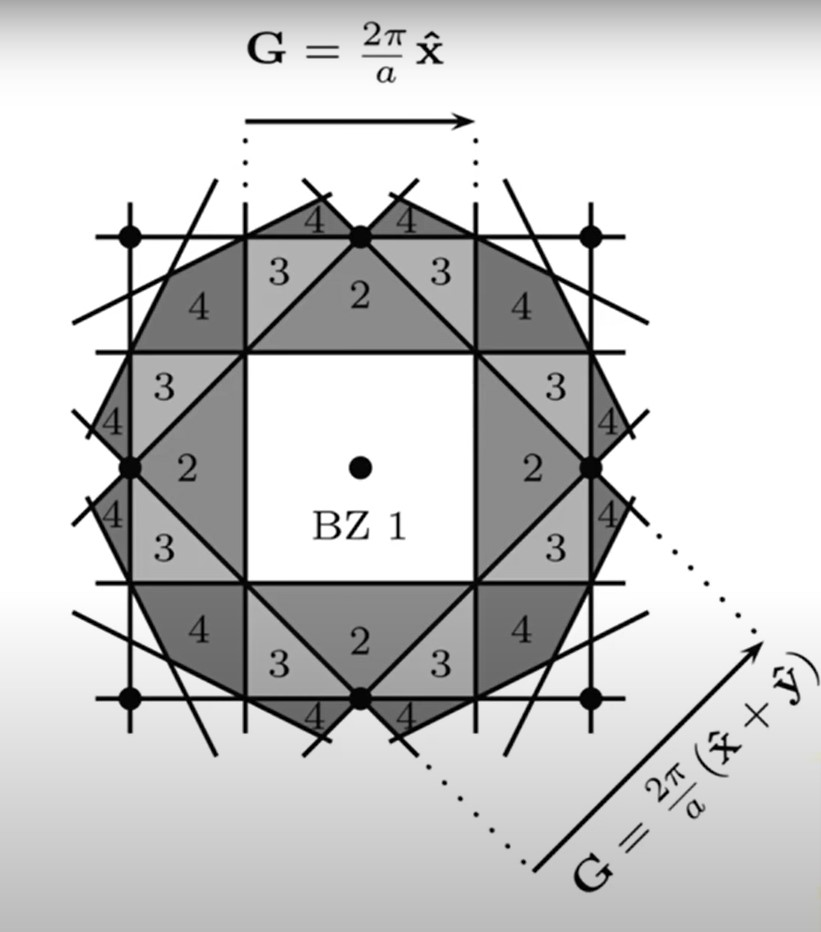
\includegraphics[width=0.75\linewidth]{Images/Bzones.jpg}
  \caption{zones}
  \label{fig:zones}
\end{figure}

- each Brillouin zone has the same area

\textbf{Band Structure in 3D}
- labelling convention to indicate points of symmetry in the Brillouin Zone. Allows us to show structure on a 2D graph.
\begin{itemize}
    \item $\Gamma$ point is the where for k=0
    \item X points at (0, 2$\pi$/a, 0)
    \item L point
    \item $\Sigma$ point
    \item $\Lambda$ point 
    \item W point 
\end{itemize}
 

\textbf{Correspondence} ==> if we start with a FCC lattice in REAL space, then RECIPROCAL lattice will be the BCC lattice.

$\therefore$

1st Brillouin Zone of an FCC lattice  = same shape as Wigner Seitz cell of a BCC lattice.

1st Brillouin Zone of a BCC lattice = same shape as Wigner Seitz cell of an FCC lattice.


- Electron and Phonon Structure can be related to the important points of the Brillouin Zone.



\textbf{Nearly-Free electron model}

- Drude and Sommerfeld models assume free electrons.
- Here we instead impose the crystal structure on a gas of free electrons (and get bands).


\[ H_0 = \frac{p^2}{2m} \]

\[E_0(k) = \frac{\hbar^2k^2}{2m} \]

- Perturbation Theory allows you to find complicated Hamiltonian solutions if we find a known similar system with solution and say there is an additional small perturbation.

 \textbf{Bloch's Theorem}
 - perturbation theory only helps if period potential is weak. 
 - Felix Bloch studied periodic potential Schrodinger equation solutions. 
 - He showed in 1928 that particles in a periodic potential will behave just like free particles except that it is their crystal momentum that is conserved in collisions rather than regular linear momentum.
 
 \begin{figure}
  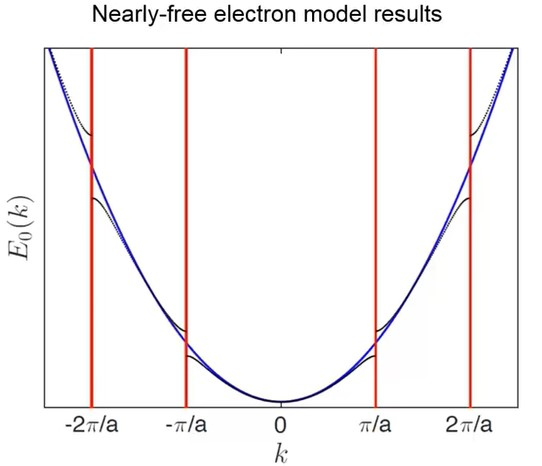
\includegraphics[width=0.75\linewidth]{Images/NearlyFree.jpg}
  \caption{nearly}
  \label{fig:nearly}
\end{figure}
 
 
 Bloch's Theorem is that a particle in a periodic potential has eigenstates of the form:
 
 \begin{tcolorbox}[enhanced,attach boxed title to top center={yshift=-3mm,yshifttext=-1mm},
  colback=blue!5!white,colframe=blue!75!black,colbacktitle=red!80!black,
  title=Bloch's Theorem,fonttitle=\bfseries,
  boxed title style={size=small,colframe=red!50!black} ]
  \begin{equation}
      \psi_\textbf{k}^\alpha (\textbf{r}) = e^{i\textbf{k}\cdot \textbf{r}}u_\textbf{k}^\alpha (\textbf{r}) 
  \end{equation}
\end{tcolorbox}

where \textbf{k} can be chosen to be within the first Brillouin zone, and the function $u_\textbf{k}^\alpha (\textbf{r})$ is a periodic function with period equal to the lattive spacing, which depends on a band index $\alpha$ and on \textbf{k}.

\textbf{- electron motion in crystals is similar to a plane waves! BLOCH WAVES! even if the electrons are strongly bound by the crystal.}


\newpage
 \section[Band Structure of Electrons in Solids]{\hyperlink{toc}{Band Structure of Electrons in Solids}}



 \textbf{Band structure representation for 1D}
 \begin{itemize}
     \item Reduced zone scheme
     \item Extended zone scheme 
 \end{itemize}

\[E = \epsilon_0 - 2J \cos(ka) \] 

- for Both we see energy band gaps

- At low temp a half filled band involves states being filled up to the Fermi Energy

- \textbf{fermi surface} is the points or planes in k where the filled meets the unfilled region

- \textbf{fermi energy} is the line in E where the filled meets the unfilled region

- \textbf{Unfilled band} allows electric field to shift electrons in band ==> conducting

- \textbf{Filled band} has no available states to move into and thus (almost) never carries a current.

- \textbf{Band filling and Fermi surfaces in 2D}

- fills up in same way $\xrightarrow{}$ lowest energy first, each level with at most one electron in each spin state.

2D hopping/tight-binding model for cubic lattic, we get energy:
\begin{equation}
    E = \epsilon_0 - 2J\cos(k_x a) - 2J \cos(k_y a)
\end{equation}


- highest unfilled band is the conduction band

- valence band is the bands that are filled.

from $\frac{p^2}{2m}$:

\textbf{lighter effective mass} $\xrightarrow{}$ sharper parabola in band

\textbf{heavier effective mass} $\xrightarrow{}$ wider parabola in band 

\textbf{Band theory does not consider interactions between electrons!} -- cannot explain:
\begin{itemize}
    \item Magnetism
    \item Mott insulators
    \item Superconductivity
\end{itemize}

- \textbf{Band insulators}: cannot absorb photons with smaller energy than the bandgap. Instead they pass through and it is transparent to them
- if BG $>$ 3.2eV, then they are transparent with visible light (ex: Quartz, diamond, sapphire (aluminium oxide).

- \textbf{Semiconductors:} smaller bandgaps can absorb for ex. violet and blue light and transmit red and green (like CdS). 
- Other smaller ($<$1.7eV) BGs may transmit in the IR but appear black cause they absorb visible light (ex. Si, Ge, GaAs).

\begin{itemize}
    \item \textbf{Direct band gap}: VB max and CB min are at the same k value.
    \item \textbf{Indirect band gap}: VB max and CB min are not at the same k value.
\end{itemize}

-indirect band gap makes it hard for material to absorb light because you need an increase in crystal momentum (which again is hard)! Not good for optical applications for lasers (but rather for electronics like silicon).



\newpage
 \section[Physics of Semiconductors (and metals and insulators)]{\hyperlink{toc}{Physics of Semiconductors (and metals and insulators)}}


- InSb is the smallest bandgap in the III-V semiconductor group


\textbf{Metals:}

- Light will excite electrons, free to move and reemit light so they look shiny.
- Conduction band width determines solver, gold, copper colour etc,

\textbf{Impurities:}

- crystal colour is effected by impurities such as Nitrogen in Diamond making it look yellow or Boron impurity making it look blue.

(area of research -- \textbf{Nitrogen-Vacancy center in diamond})

- or oxides (insulator) on shiny metal (conductor) can make it look matte.

\textbf{Basic Properties of Semiconductors}


\textbf{Electrons and Holes:}
\begin{itemize}
    \item semiconductor with filled VB and excite one electron to the conduction band (photon absorption or thermal excitation).
    \item \textbf{Hole} is then the absence of an electron in VB.
\end{itemize}

 
 \begin{figure}
 \centering
  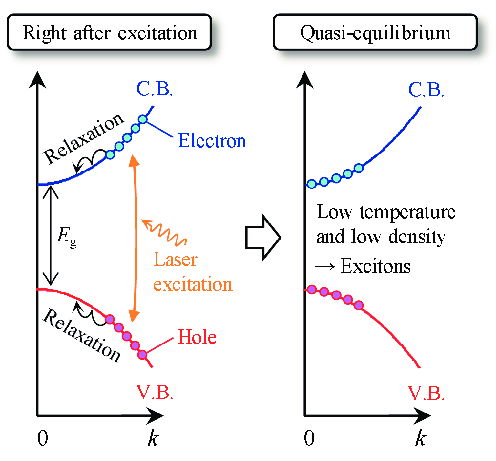
\includegraphics[width=0.75\linewidth]{Images/electron-holes.png}
  \caption{electronholes}
  \label{fig:electronholes}
\end{figure}

\textbf{Holes}
\begin{itemize}
    \item convenient to keep track of the holes 
    \item effectively act like a positive charge
    \item moves like a particle
    \item has charge and mass
    \item not a real particle $\xrightarrow{}$ only a quasi-particle
    \item electrons here with effective mass are actually also quasi-particles
    \item electron and hole pair attract each other and for another quasi-particle called an exciton
    \item exciton is a Boson because it is composed of two Fermions (electon and holes). (bose-einstein condensate is a field of research that is not covered in the course).
    \item electron can fall back, "annihilating" the conduction electron and the hole in the valence band (analogous to electron-positron, particle-antiparticle pair).
    \item convention to make mass of hole positive, since it takes energy to accelerate the hole from zero vel to finite vel (like pushing a balloon underwater).
\end{itemize}


\begin{equation}
    \frac{\hbar^2}{m_h^*} = -\frac{\partial ^2E}{\partial k^2} = 2 \alpha
\end{equation}

\textbf{How to Measure the Effective Mass}

- Cyclotron Resonance Technique
\[F = \frac{mv^2}{r} = qvB\]

\[ f = \frac{qB}{2\pi m} \]

- independent or v and r 

- electrons strongly absorb microwaves of that frequency

- only need to measure freq to solve for effective mass.



\begin{tabular}{ |p{1.5cm}|p{1.5cm}|p{1.5cm}|p{1.5cm}|p{1.5cm}|p{1.5cm}|  }
 \hline
 \multicolumn{6}{|c|}{\textbf{Electron and hole effective masses}} \\
 \hline
    & Si & Ge & GaAs & InAs & AlAs\\
 \hline
 $m_n/m_0$ & 0.26 & 0.12 & 0.068 & 0.023 & 2 \\
 $m_p/m_0$ & 0.39 & 0.3 & 0.5 & 0.3 & 0.3 \\
 \hline
\end{tabular}

\textbf{Doping Semiconductors}
\begin{itemize}
    \item pure ins. or semcond. excite electrons from VB to CB and the density of electrons in the conduction band (n for negative charges) is equal to the density of holes in the valence band (p for positive charges).
    \item \textbf{Intrinsic:} semiconductor without impurities
    \item \textbf{Extrinsic:} when impurities are placed in the SC
\end{itemize}



\textbf{Intrinsic Carrier Concentration:}

\begin{itemize}
    \item Density of States (DoS): how many eigenstates at each energy. 
\end{itemize}

 \begin{tcolorbox}[enhanced,attach boxed title to top center={yshift=-3mm,yshifttext=-1mm},
  colback=blue!5!white,colframe=blue!75!black,colbacktitle=red!80!black,
  title=Law of Mass Action,fonttitle=\bfseries,
  boxed title style={size=small,colframe=red!50!black} ]
  \begin{equation}
      np = 4\left(\frac{1}{2\pi\hbar^2\beta}\right)^3(m_em_h)^{3/2}e^{-\beta E_g}
  \end{equation}
\end{tcolorbox}

 intrinsic carrier concentration -- Fermi level is inside the gap and the density of holes and electrons are equal then each density is the sqrt of the above expression on the right.
 
 
 It is often useful to intentionally add impurities.
 
 Consider:
 \begin{itemize}
     \item silicon a semiconductor with a bandgap of 1.1eV
     \item replace one atom with phosphorus (which has one extra proton and one extra electron)
     \item VB is filled and so electron must go into the conduction band
     \item known as donor, \textbf{electron donor}, or \textbf{n-dopant}, as n is the symbol from the density of electrons in the conduction band.
 \end{itemize}
 
 or instead:
 \begin{itemize}
     \item replace one atom with Aluminium
     \item provides one fewer electron than silicon
     \item missing electron from the VB, leaving a hole.
     \item known as \textbf{electron acceptor}, or a \textbf{p-dopant}
 \end{itemize}
 
 - semiconductor Fermi energy is in the middle of the band gap, and then dopants shift it up for n-dopant case and down for the p-dopant case. 


\newpage
\section[Graphene and Carbon Nanotubes]{\hyperlink{toc}{Graphene and Carbon Nanotubes}}

 
 \begin{itemize}
     \item Carbon is versatile in bonding with other atoms
     \item Carbon is responsible for all organic chem
     \item Graphite (like in pencils) most closely related to Graphene
     \item 2 atom basis, FCC
     \item pencils (Graphite) are able to write because you can remove one layer (Graphene) at a time quite easily since each layer is bonded with van der Wall forces only.
     \item Graphene is single hexagonal lattice (not technically a lattice since you can't get to all points with primitive vectors) is exceptionally strong
     \item Konstantin Novoselov (Manchester) first to get graphene from scotch tape.
     \item colour change indicated that they had gotten to a monolayer
     \item solution to the graphene hamiltonian is found with tight binding mode, and my spliting the atoms up into 2 groups of triangular lattices. 
     \item \textbf{K and K'} points: where the 2 bands meet each other and touch (no energy gap)
     \item two seas of electrons but they can't get to each other (K and K' points are separate and different).
     \item semiconductor has a small bandgap, but graphene has filled valence band and empty conduction band, but the two bands are touching and thus it is considered and metal.
     \item the dispersion relation where it touches is called a Dirac Cone (ex Graphene)
     \item area of research here is called "klein tunneling"
     \item Electrons have extremely fast fermi velocity $v_F = 8E5 m/s$.
 \end{itemize}
 
 \textbf{Carbon Nanotubes!} - rolled up graphene
 
 \begin{itemize}
     \item Bonds on edge of graphene are happier if rolled around and connected to the other edge (forming a tube).
     \item can "roll" the graphene in different orientations
     \item for ex: armchair (up-flat-down), zig-zag (up-down), and chiral (various wrapping).
     \item Carbon Nanotubes (depending on the rolling vector) can "gap" Graphene (which is normally gapless.
     \item Armchair (n,n): $\theta=30$ always Metal
     \item Zig Zag (n,0): $\theta = 0$ then 2/3 are Metal and 1/3 are Semiconductor (for n multiples of 3)
     \item Chiral (n,m): $0<\theta<30$, 2/3 are meteal, and 1/3 are semi-conducting, n-m multiple of 3.
 \end{itemize}
 
 It turns out that there is a formula which tells us if the carbon nanotube will be conducting or not (i.e. if it won't hit the K point)
 
 \begin{equation}
     2n_1+n_2 = 3m \qquad m\in \{1,2,3, ...\}
 \end{equation}


\newpage
\section[Semiconductor Devices]{\hyperlink{toc}{Semiconductor Devices}}



\textbf{Heterostructures}: Layers of 2 or more different semiC - band strucutre design.


Lattice mismaatch negligile -- heterojunction = single crystal with different site occupancies across juntion.


3 types of band edge offsets:
\begin{enumerate}
    \item Normal
    \item Staggered
    \item Broken Gap
\end{enumerate}

\begin{itemize}
    \item To make a clean growth of heterostructures you want to match lattice constants (a) very closely
    \item if it is not matched you will get strain in your sample, and you will get deffects in your grown sample.
    
    \item \textbf{Transmission Electron Microscope (TEM):} send electrons at very high energy all the way through the structure, and pixels represent atomic rows. tells you about the crystallinity of the structure under study.
    
    \item \textbf{Molecular Beam Epitaxy (MBE)}: The structures are gorwn in MBE machines. It generates beams of molecules, and grow layer by layer (epitaxially). 
    \item Stainless steal \textbf{ultra high vacuum chamber} so that beams of molecules can go in straight lines and not collide with anything (massive mean free path).
    \item \textbf{Diffusion cells} (molecular guns): buckets containing different materials, heated to a certain temperature where material begins to sublimate.
    \item \textbf{Substrate} is the base on which you grown an epitaxial thin film.
    \item Overlap of for ex. Ga and As shooting at the same time onto the substrate allows for growth of GaAs.
    \item \textbf{ Reflection High Energy Electron Diffraction (RHEED):} Shoots electrons at sample which reflect and hit screen while the sample is being grown. Intensity of diffraction pattern oscillates as you're growing. Used to count the layers grown so far.
    \item RHEED: max diffraction pattern intensity at new layer, min at half layer, max at completion of a layer. layer by layer we can see and count the layers that have been grown so far.
    \item \textbf{Quantum Wells:} \begin{equation}
        E = n^2 \frac{\hbar^2 \pi^2}{2m_eL_z^2} \qquad \in n =1,2,3.
    \end{equation} 
    \item \textbf{Gas LASER:} for ex HeNe works on the atomic transitions within the gas, and uses some kind of pump to bring all the atoms into the excited state and they relax and emit photons all with the same energy. usese mirror structure to boost this process.
    \item \textbf{Quantum Well Laser (27:00):} pumping by sending electrical current through. 
    \item \textbf{Quantum Cascade Laser:} electrons falls from one QW to the next each time emitting a photon of a specific energy.
    \item \textbf{Field Effect Transistor (HEMT- High electron mobility transistor):} 3 components - source, gate and drain
    \item \textbf{2DEG: Two Dimensional Electron Gas}
    \item \textbf{PN Junction (Diode):} When N-type and P-type dopants are introduced side-by-side in a semiconductor, a PN junction or diode is formed. \item \textbf{Rectifier Circuits:} converts an AC voltage into a DC voltage.Sin wave negative values are cut off by diodes unidirectional feature. 
    \item \textbf{Light Emitting Diodes (LED):} Recombination in the middle of the PN junction diode of the electron and hole emits a photon. Band gap of the junction determines the colour of the photon.
    \item Blue LEDs won a nobel prize recently with nitride based diodes.
    \item \textbf{Bandgap Engineering:}
    \begin{figure}
    \centering
    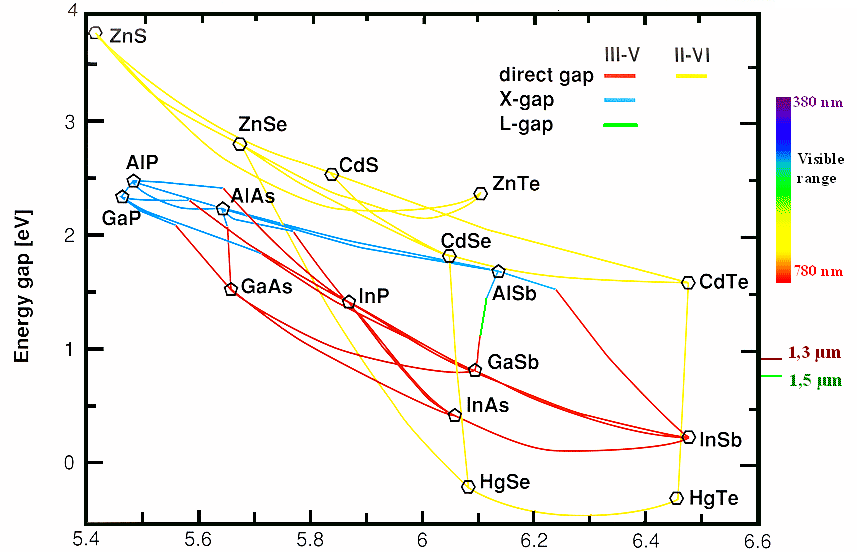
\includegraphics[width=0.75\linewidth]{Images/bandgap_misfit.png}
    \caption{bandgap}
    \label{fig:bandgapengineering}
    \end{figure}
    Tweaking structures to tune the wavelength and the properties.
    \item \textbf{Solar Cells:} Photon comes in and excites an electron-hole pair in a PN junction. The charges separate and this produces a current.
    \item \textbf{Schottky Barrier:} Metal-SemiC Junction.
    \item \textbf{Metal-Oxide-Semiconductor Transistors:} Most modern digital devices use MOS transistors. Greater density and simpler geometry (easier to make). Switch on and off more slowly. 
    \item Consists of source, drain diffusions, with a gate that controls whether the transistor. 
    \item MOSFET: Metal-Oxide Semiconductor Field Effect Transistor.
    \item Applying positive gate voltage (attracts electrons to gate area, i.e. a conductive path),causes current to flow from source to drain. The more voltage, the more current.  
    \item negative current in MOSFET is like two diodes facing each other (both directions blocked).
    \item \textbf{Complementary MOS Transistors:} Use transistors for logic circuits.
    \item \textbf{Integrated Circuit (IC) chips:} 12 inch semiC wafer printed at INTEL with nanofabrication. out of silicon with n and p doped regions and metal contacts. chopped up into chips to be put into our laptops. They are filled with hundreds of millions of MOSFETS.
    \item \textbf{Electric Field in a CCD:} Charge coupled device. Pixel in our digital camera. Also functions with a P-N junction.

\end{itemize}

\newpage
\section[Paramagnetism and Diamagnetism]{\hyperlink{toc}{Paramagnetism and Diamagnetism}}


\textbf{General}
\begin{itemize}
    \item original data storage devices
    \item only started to understand micro level after advent of QM
    \item goes past band structure
    \item treat interactions between particles
    \item interactions between spins are fundamental to current research: spintronics + quantum technologies using spins.
    \item phase transitions
\end{itemize}

\textbf{Spinors}

\begin{equation}
    \alpha \ket{\uparrow} + \beta \ket{\downarrow} = \begin{pmatrix}
    \alpha  \\ \beta
    \end{pmatrix}, \qquad |\alpha|^2 + |\beta|^2 = 1
\end{equation}
\begin{equation}
    S_z = \frac{1}{2} \hbar \sigma_z, \qquad \sigma_z = \begin{pmatrix} 1 & 0 \\ 0 & -1 \end{pmatrix}
\end{equation}

\textbf{Bloch sphere representation}
\begin{equation}
    \ket{\Psi} = \cos{\frac{\theta}{2}}\ket{\uparrow} + \sin{\frac{\theta}{2}}e^{i\phi}\ket{\downarrow}
\end{equation}

\textbf{Magnetic Susceptibility}
\begin{equation}
    M = \chi \frac{\textbf{B}}{\mu_0}
\end{equation}

 \begin{tcolorbox}[enhanced,attach boxed title to top center={yshift=-3mm,yshifttext=-1mm},
  colback=blue!5!white,colframe=blue!75!black,colbacktitle=red!80!black,
  title=Bohr-van Leeuwen Theorem,fonttitle=\bfseries,
  boxed title style={size=small,colframe=red!50!black} ]
  \begin{equation}
      \braket{\textbf{M}} = \braket{\lambda \textbf{L}} = 0, \qquad \text{according to classical statistics} \rightarrow \text{magnetism obeys quantum statistics}
  \end{equation}
\end{tcolorbox}

\textbf{Properties of Magnetism can have three origins,}
\begin{itemize}
    \item Intrinsic angular momentum (Spin). 
    \item Orbital angular momentum about the nuleus
    \item Change in the dipole moment due to an applied magnetic.
    
    \item When electrons are \textbf{paired together} their opposite spins cause their magnetic fields to cancel each other. Therfore, \textbf{no net magnetic field exists}. Alternatively, materials with some \textbf{unpaired electrons} will have a \textbf{net magnetic field} and will \textbf{react} more to an \textbf{external field}.
\end{itemize}

\textbf{Hund's Rules (L-S coupling scheme -- how to fill up orbitals in atoms):}
\begin{itemize}
    \item Outer shell electrons of an atom in its ground state should assume:
    \begin{enumerate}
        \item Max Value of S (spin momentum) allowed by exclusion princple.
        \item Maximum value of L (orbital momentum) compatible with (1).
        \item $J=|L-S|$ for less than half-filled shells. \\$J = L+S$ for more than half-filled shells.
        
        Causes: 
        $
        \begin{cases}
        \text{parallel spins have lower Coulomb energy.}\\
        \text{e's meet less frequently if orbiting in same direction (parallel Ls).} \\
        \text{Spin orbit coupling lowers energy for} + L*S < 0
        \end{cases}
        $
    \end{enumerate}
    
    \item examples:\\
    $
    \begin{cases}
    \text{Mn}^{2+}: \qquad 3d^5 \qquad (1) \rightarrow S=5/2 \qquad \text{excl. princ.} \rightarrow L = 2+1+0-1-2 = 0 \\
    \text{Ce}^{3+}:\qquad 4f^1 \qquad L = 3, S = \frac{1}{2} \qquad (3) \rightarrow J = |3-\frac{1}{2}| = 5/2 \\
    \text{Pr}^{3+}: \qquad 4f^2
    \qquad (1) \rightarrow S = 1 \qquad (2) \rightarrow L = 3+2 = 5 \qquad (3) \rightarrow J = |5-1|=4
    \end{cases}
    $
    \item shell filling structure is important
\end{itemize}

\textbf{Paramagnetism (positive suceptibility):}
\begin{itemize}
    \item a paramagnet has a response that tends to enhance the applied field, i.e., \textbf{$\chi > 0.$}
    \item This is usually due to the spin of the \textbf{unpaired electrons} fixed within the crystal.
    \item the simplest model for p.m. (known as \textbf{Currie Paramagnetism} after Pierre Curie, or Langevin Paramagnetism) is the result of considering a collection of non-interacting spin-1/2 particles.
    \item Occurence of electronic paramagnetism:
    \begin{itemize}
        \item Atoms, molecules, and lattice defects with \textbf{odd numbers of electrons} (S $\neq$ 0).
        E.g., Free sodium atoms, gaseous NO, F centers in alkali halides, organic free radicals such as $C(C_6H_5)_3$
        \item Free atoms and ions with \textbf{partly filled inner shell} (free or in solid), E.g., Transition elements, ions isoelectronic with transition elements, rare earth and actinide elemnts such as $\text{Mn}^{2+}\text{, Gd}^{3+}\text{, U}^{4+}.$
        \item Only a few compounds with even number of electrons, E.g. $O_2$, organic biradicals.
        \item \textbf{metals}
    \end{itemize}
    \item For a free spin-1/2 particle, the Hamiltonian is given by the so called the Zeeman Term:
    \[ H = g \mu_B \textbf{B}\cdot \vec{\sigma} \]
    where $g=2$ is the g-factor for the electron, $\vec{\sigma}$ is an operator for the spin and $\mu_B = e\hbar/(2m) \approx 0.67k_B $ Kelvin/Tesla is the Bohr Magneton.
    \item The single spin can be oriented either parallel or antiparallel to the field, so the energies for the two states of a single spin can be:
    \[ E = \pm \mu_B B \]
    \item Then we know that the probabilities of the two states are given by:
    \[p_{\uparrow} = \frac{e^{-\beta \mu_B B}}{Z}, \qquad  p_{\downarrow} = \frac{e^{+\beta \mu_B B}}{Z}, \qquad Z = e^{-\beta \mu_B B}+ e^{+\beta \mu_B B}\]
    where $\beta = 1/(k_B T) $
    \item Zeeman Splitting
    \item 36:00min derivation to get susceptibility:
    \[ \chi = \frac{\mu_0 \mu_B^2}{k_B T}\]
    and for a collection of spins with density n we then have 
    \[\chi = \frac{n \mu_0 \mu_B^2}{k_B T} \]
    \item Result: \textbf{Magnetization increases as you lower the temperature: Currie Law susceptibility is dependence on $1/T$}
\end{itemize}

\textbf{Paramagnetic Susceptibility of Conduction Electrons:}
\begin{itemize}
    \item Classical free electrons: $M \approx \frac{N \mu^2 B}{k_B T} \qquad \sim$ Curie paramagnetism
    
    \item Experiments on normal non-ferromagnetic metals: M independent of T
    
    \item Pauli's resolution: Electrons in Fermi sea cannot flip over due to exclusion principle. Only fraction $T/T_f$ near Fermi level can flip.
\end{itemize}

\textbf{Pauli Paramagnetism}
\begin{itemize}
    \item For some alkali metals and noble metals, conduction electrons are weakly interacting and delocalized in space forming a Fermi gas. For these materials one contribution to the magnetic response comes from the interaction between the electron spins and the magnetic field known as Pauli paramagnetism. 
    \item The Pauli paramagnetic susceptibility is a macroscopic effect and has to be contrasted with Landau diamagnetic susceptibility which is equal to minus one third of Pauli's and also comes from delocalized electrons. The Pauli susceptibility comes from the spin interaction with the magnetic field while the Landau susceptibility comes from the spatial motion of the electrons and it is independent of the spin. In doped semiconductors the ratio between Landau's and Pauli's susceptibilities changes as the effective mass of the charge carriers $m^{*}$ can differ from the electron mass $m_{e}$.
    
    \item Before Pauli's theory, the lack of a strong Curie paramagnetism in metals was an open problem as the leading Drude model could not account for this contribution without the use of quantum statistics. Pauli paramagnetism and Landau diamagnetism are essentially applications of the spin and the free electron model, the first is due to intrinsic spin of electrons the second is due to their orbital motion.
\end{itemize}

\textbf{Diamagnetism}
\begin{itemize}
    \item can come from orbital mechanism in a Free Electron Gas (not going to talk much about it)
    \item or from a fully filled shell
    \item famous example is frog floating in a magnetic field (diamagnetism)
    \item phenom characterized by negative susceptibility ($\chi<0$).
    \item appears in most materials but is often dominated by other effects
    \item superconductors tend to be good diamagnets
    \item main type is called Larmor diamagnetism (comes from Larmor Precession) when other magnetic effects are not present.
    \item Need J=0 otherwise Curie Paramagnetism dominates
    \item relates in Lenz's Law
    \item you can also use paramagnets to make an adiabatic demagnetization refrigerators
\end{itemize}


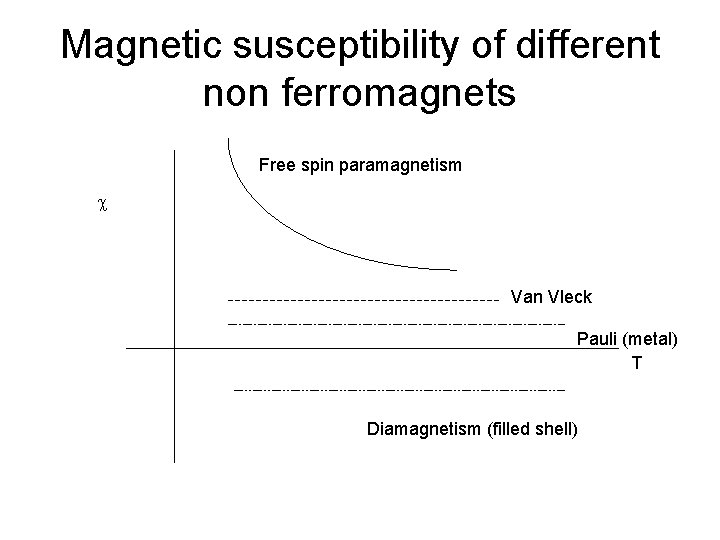
\includegraphics[width = \linewidth]{Images/paramagnetism.jpg}




\newpage
\section[Magnetic Order]{\hyperlink{toc}{Magnetic Order}}

\begin{itemize}
    \item spontaneous or under the infl of some \textbf{interactions}: all the spins line up in the same direction even without an external magnetic field
    \item ex. ferromagnet, antiferromagnet, and ferrimagnet.
    \item best ex of ferromagnet is Iron
    \item above a particular temp, spins tend to align randomly and there is a transition at the so called Curie Temperature to a paramagnetic behaviour.
    \item spin in the same direction reduces the energy and so is favourable for the system
    \item Spin-Spin interactions of localised spins we have the \textbf{Heisenberg Hamiltonian}
    \[ -J \sum_{\braket{i,j}}  \textbf{S}_i \cdot \textbf{S}_j , \qquad J>0\]
    and $\textbf{S}_i$ is the spin operator for the ith spin and $\braket{i,j}$ denotes the sum over all neighbouring spins.
    \item Also \textbf{Antiferromagnet} ordered at low Temp, but with zero magnetisation.
    \item discovered by Louis Neel in the 1930s (thus we get Neel Order).
    \item \textbf{Heisenberg Hamiltonian} is very similar but without the negative sign:
    \[ J \sum_{\braket{i,j}}  \textbf{S}_i \cdot \textbf{S}_j , \qquad J>0\]
    \item i.e. alternating spins (up-down-up-down-...) results in minimizing the energy.
    \item if the lattice is triangular you get a \textbf{frustrated magnet} because there are lattice sites that you cannot optimize the lowest energy very well. i.e. think of triangular lattice.
    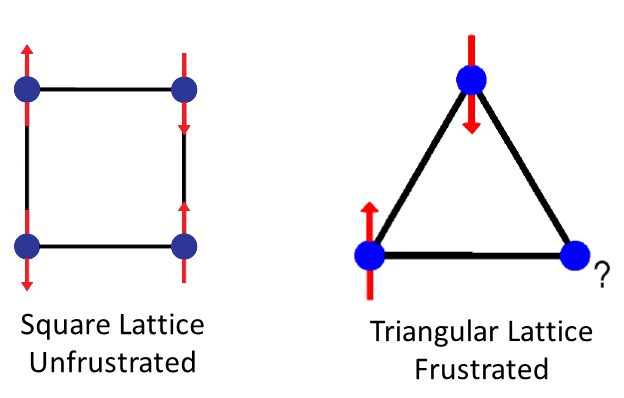
\includegraphics[width= 0.5\linewidth]{Images/Frustration.png}
    \item \textbf{Ferrimagnetism}: 'weak form of ferromagnetism', spins allign within one sublattive but oppose each other on other sublattices. Normally a net magnetic field but typically weaker.
    
    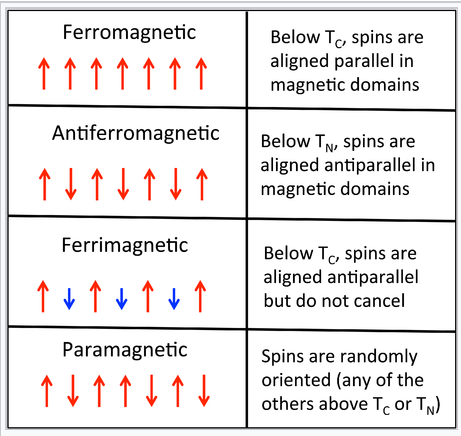
\includegraphics[width = 0.5 \linewidth]{Images/magnetic order.png}
    
    \item Also possible order called canted antiferromagnet and helical spin array.
    
    \item How to detect magnetic order?
    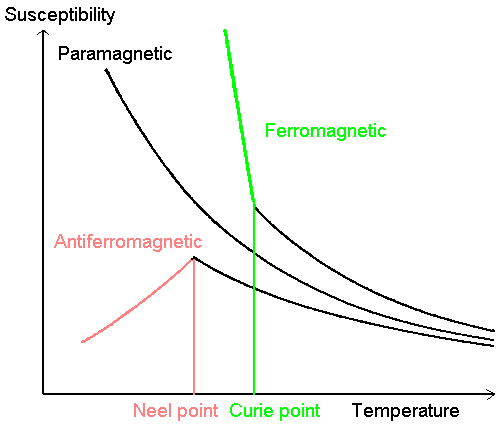
\includegraphics[width  = 0.5 \linewidth]{Images/magnetic chemistry.png}
    \item Measure how magnetic susceptibility changes as you decrease the temperature. Find possible critical temperatures to see deviant behaviour. At high temps they all behave like a paramagnet.
    \item Neutron Scattering Experiment (neutrons have spin): the moments of the neutrons will overlap with the atoms. Interactions with the spin up atoms will be different than the spin down atoms. So you can measure the lattice spacing between spin up or down atoms and see how it increases or decreases with decreasing temperatures. This can show you if it became antiferromagnetic (bigger lattice constant, that is between the atoms of the same spin) or ferromagnetic (smaller lattice constant).
    
    \item \textbf{Domains and Hysteresis:}
    \item \textbf{Annealing}: to make a ferromagnet, hold it at a high temperature and slowly lower the temperature while applying a strong magnetic field in one direction.
    \item \textbf{Magnetic domains} separated by \textbf{domain walls}: If it is cooled down too quickly or the field is too weak, then symmetry can be broken differently in different regions.
    \item \textbf{Quench}: Changing a parameter such as temperature quickly across a transition.
    
    \item Domain walls normally occur over a small region and involve the spin gradually rotating from the value of one domain to that of another (energy is minimized). We then have the bloch (rotation through the plane) and neel (rotation in the plane) walls:
    
    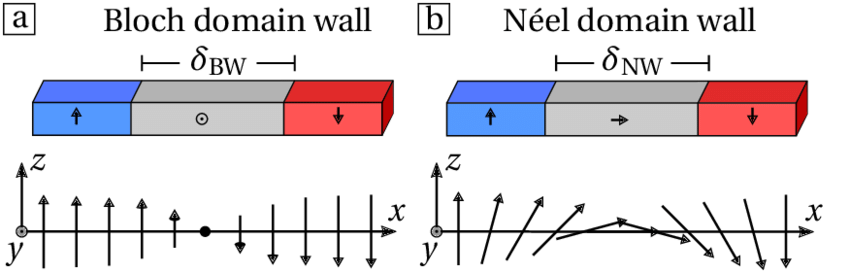
\includegraphics[width = 0.9\linewidth]{Images/domain walls.png}
    
    \item For instant change we get an energy cost of: $\Delta U = JS^2 $
    
    \item For a domain wall of finite width we get: $\Delta U = JS^2 (1- \cos\theta), \quad \theta = \frac{\pi}{N}$ since the spins change by 180 degrees in N spin steps. If we only consider this it would seem the wall would extend to infinite. Therefore we find an extra anisotropy term:
    
    \[ \Delta U = +JS^2 \frac{N}{2} \left( \frac{\pi}{N} \right)^2 + KN \]
    
    Where K = anisotropy term
    \item Average width of the wall is around 150 lattice constants for iron and other ferromagnets.
    
    \item Size of domains walls can be seen as a trade off between energy cost of spins not being aligned (worse if the interactions are stronger), and the preference of the crystal to have particular spin directions (not diagonal: the anisotropy energy).
    
    \item \textbf{Domain wall pinning}: tendency of domain walls to intersect where the defects are in the crystal to minimize the overall energy.
    
    \item \textbf{"Hard Ferromagnet" = Nonzero Hysteresis Loop}.
    
    We observe hysteresis in magnetic susceptibility -- there is typically residual magnetisation when the field is changed.
    
    \item \textbf{Magnetic Force Microscopy (MFM):} Resolution ~ 10-100 nm
    
    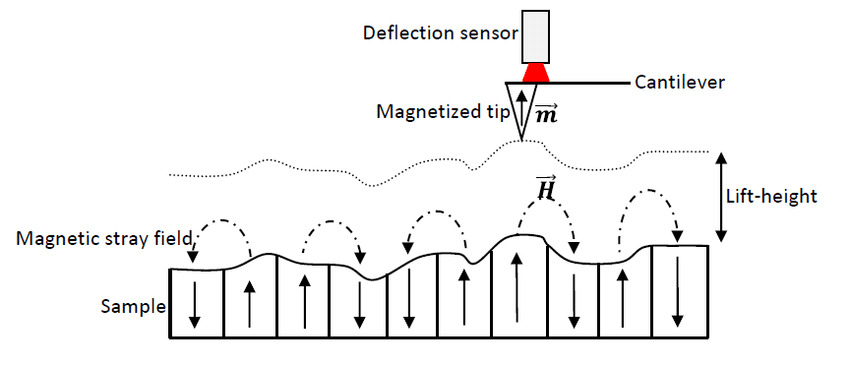
\includegraphics[width = 0.9\linewidth]{Images/MFM.jpeg}
    
    \item Also Atomic Force Microscope (AFM) used for non magnetic samples. Can identify individual atom lattice sites if tuned well. External vibration frequency from the cantilever removes noise (mechanical lock-in technique).
    
    \item Many Types of Resonance Phenomena/ Instruments
    
    \item \textbf{Information Gained:}
    \begin{itemize}
        \item Fine structino of absorption: Electronic structure of individual defects.
        \item Change in line width: Motion of the spin or its surroundings
        \item Chemical or Knight shift: Internal Magnetic field felt by the spin.
        \item Collective spin excitations.
    \end{itemize}
    
    \textbf{Main Applications with Nuclear Magnetic Resonance:} 
    \begin{itemize}
        \item Identification and structure determination for organic / biochemical co
        \item Medical (MRI)
    \end{itemize}
    
    \item \textbf{NMR}:
    
    Nucleus with a magnetic moment \textbf{$\mu$} and angular momentum \textbf{I}.
    
    \[\mu = \gamma \hbar I, \qquad \gamma = \textbf{gyromagnetic ratio} \]
    
    Resonance at:
    
    \[\omega_0 = \gamma B_0 \]
    
    \item Signal Detection (via RF coil)
\end{itemize}


\newpage
\section[Mean Field Theories of Magnetism]{\hyperlink{toc}{Mean Field Theories of Magnetism}}

The Ising Model
Goal: Get Magnetization as a function of Temperature and Magnetic Field; $M(T,B)$
\begin{itemize}
    \item If we forget about spin interactions, Spins within a lattice will act as a paramagnet and try to align with an external field.
    \[H_{p} = \sum_l  g \mu_B \vec{B} \cdot \vec{\sigma_l}\]
    And can be simplified if we consider a given field direction.
    \item We also can take into account the interactions between nearest neighbouring spins within a 2D lattice (summation will double counting, so divide by 2 on the outside):
    \[H_{int} = -\frac{J}{2}\sum_{<i,j>} \sigma_i \sigma_j \]
    \item if $J>0$ this is a ferromagnet and for $J<0$ this would be an antiferromagnet.
    \item Ising grad student solved it in 1D (1925). And in 2D by Onsage (1945). Only solvable in 3D with more approximations (mean field theory approach). The combination of the two interactions that the Ising Model considered is:
    \[H_{Ising} = g \mu_B B \sum_l \sigma_l - \frac{J}{2} \sum_{<i,j>} \sigma_i\sigma_j\]
\end{itemize}

\textbf{Mean-field theory for the Ising Model:}
\begin{itemize}
    \item Single out a subset of the system and then treat interactions with all other parts of the system as some sort of potential. In a sense averaging out all the interactions will give you the mean field.
    \item Self-consistent result that is useful for a large number of particle systems.
    \item Focussing on one spin at site i, the Hamiltonian is:
    \[H_{i} = g \mu_B B \sigma_i - J \sigma_i \sum_{j\in N_i} \sigma_j\]
    summing over all j that are nearest neighbours of i.
    \item Next, we instead use the average over all the neighbours of i:
    \[H_{i} \approx g \mu_B B \sigma_i - J \sigma_i \sum_{j\in N_i} \left<\sigma_j\right>\]
    \item Solution gives us the transcendental equation which we can solve numerically or graphically:
    \[\langle\sigma_i\rangle = \frac{1}{2} \tanh \left(\frac{ \beta J z \langle\sigma_i\rangle}{2}\right)\]
    \item Solution shows that when T is large (small $\beta$) the curves only intersect at $\langle\sigma_i\rangle=0$ so that there is no average magnetization. 
    \item When T is small, we enter a regime where curves intersect at three points. This shows spontaneous magnetization.
    \item transition point between two behaviours happens when slopes are the same at small $\langle\sigma_i\rangle$
    \item Make some simplifications and get a critical temperature:
    \[T_c = \frac{J_z}{4k_B}\]
\end{itemize}

\textbf{(Spontaneous) Symmetry Breaking}
\begin{itemize}
    \item Free energy of the system as we pass through the $T_c$. Using $F = -k_B T \log Z$, we can compute this function as a function of $\langle \sigma_i\rangle$ from the partition function.
    \item parabola (with min at 0) changes to camelback (with 2 mins on either side of 0, and a hump at 0) after going past $T_c$, the middle hump is an unstable point and system will lower energy by breaking symmetry and going to a non-zero magnetization -- i.e. spontaneously polarize.
    \item Applying an external field explicitly breaks the symmetry and we can determine  the directions in which the spins align.
    \item to Make Permanent Magnet from Iron: Heat above $T_c$, align with a strong field, then cool to a temperature below $T_c$.
\end{itemize}

\textbf{Itinerant Ferromagnetism}
\begin{itemize}
    \item Ising model said spins are fixed and can only interact; now this model spins can also hop (and still interact with each other).
    \item electrons tend to exhibit this behaviour
    \item The \textbf{Hubbard Model} describes electrons that hop through a tight-binding lattice, combined with interactions that occur if two electrons si on the same site of the lattice.
    \item Tunnelling amplitude J (not same as Ising), and interaction energy if 2 electrons are on the same lattice site, U.
    \[H_{interaction} = \sum_i U n_{i\uparrow} n_{i\downarrow}\]
\end{itemize}



\newpage
\section[Superconductivity Experiments]{\hyperlink{toc}{Superconductivity Experiments}}

\begin{itemize}
    \item Interesting topic because we get neat phenomena like R=0, and also quantum mech application.
    \item Lecture is survey on superconductivity and why it is different 
    \item Not just band theory (fails here), need to account for interactions between electrons.
\end{itemize}

\textbf{Heat capacity of Solids}

\begin{itemize}
    \item Heat capacities at constant volume are defined as the rate of change of energy with temperature.

    \[ C = \frac{dE}{dT}\]

    \item at high temperature, $C=3Nk$, where N is the number of atoms in the solid and k is Boltzmann's constant (law of Dulong and Petit).

    \item Understood classically from the law of equipartition, which assigns a heat capacity of $k/2$ to each degree of freedom in the material.
\end{itemize}

\textbf{Temperature dependence of Resistivity}

\begin{itemize}
    \item Metal: for a sufficiently narrow range of temperature, make a linear approximation:

    \[ \rho(T) = \rho_0 [1+\alpha(T-T_0)]\]

    where $\alpha$ is the temp coefficient of resistivity, $T_0$ is a reference coefficient of resistivity, and $\rho_0$ is the resistivity at temperature $T_0$. 

    \item Standard resistivity of metal changes with temp. 
    
    \item Electrons in fermi gas occupy metal.

    \item 
\end{itemize}


\newpage
\input{Lectures/21_Physics_of_Low-Dimension_Systems:_2D}

\end{document}